\documentclass{article}
\usepackage[utf8]{inputenc}
\usepackage[papersize={8.5in,11in},margin=0.8in]{geometry}
\usepackage{xcolor}
\usepackage{color, colortbl}
\usepackage{graphicx}
\usepackage{tikz}
\usepackage{amssymb}
\usepackage{amsmath}
\usetikzlibrary{positioning}
\usetikzlibrary{graphs,graphs.standard}


\title{MATH 505 HW 8}
\author{John Caruthers}
\date\today

\begin{document}
\maketitle

\textbf{Section 4.1}

\begin{itemize}
    
    \item[5.] The Highway inspector problem was first solved by Leonhard Euler in 1735 when thinking about a puzzle problem that he describes as follows: "In the town of Konigsberg there is an island called Kneiphof, with two branches of the river Pregel flowing around it.  There are seven bridges crossing the two branches.  The question is whether a person can plan a walk in such a way that he wil cross each of those bridges once but not more than once." Redraw this as a map with $A, B, C,$ and $D$ representing towns and the bridges representing sections of road. Can you answer Euler's puzzle?
    
    \begin{center}
        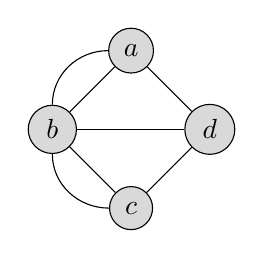
\begin{tikzpicture}
           [dot/.style = {draw,fill=gray!30,circle}]
            \node[dot] (a) at (0, 0) {$a$};
            \node[dot] (b) at (-1,-1) {$b$};
            \node[dot] (d) at (1,-1) {$d$};
            \node[dot] (c) at (0,-2) {$c$};
        
            \path[-] (a) edge (b);
            \path[-] (b) edge (c);
            \path[-] (c) edge (d);
            \path[-] (d) edge (a);
            \path[-] (b) edge (d);
            \path[-] (a) edge[out=180,in=90] (b);
            \path[-] (b) edge[out=270,in=180] (c);
            
            \end{tikzpicture}
    \end{center}
    
    {\color{blue} There is no Euler path since there are more than two odd nodes.}
    
    \item[6.] A city is built along both sides of a river and includes three islands $A, B, C$ and nine bridges as shown.  Is it possible to walk around the city and cross each bridge exactly once?
    
    \begin{center}
        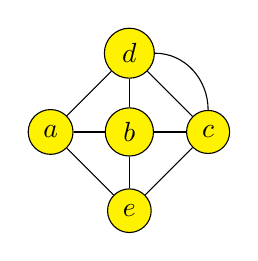
\begin{tikzpicture}
           [dot/.style = {draw,fill=yellow,circle}]
            \node[dot] (d) at (0, 0) {$d$};
            \node[dot] (a) at (-1,-1) {$a$};
            \node[dot] (c) at (1,-1) {$c$};
            \node[dot] (e) at (0,-2) {$e$};
            \node[dot] (b) at (0,-1) {$b$};
        
            \path[-] (d) edge (a);
            \path[-] (a) edge (e);
            \path[-] (e) edge (c);
            \path[-] (c) edge (d);
            \path[-] (a) edge (b);
            \path[-] (d) edge (b);
            \path[-] (c) edge (b);
            \path[-] (e) edge (b);
            \path[-] (d) edge[out=0,in=90] (c);
            
            \end{tikzpicture}
    \end{center}
    
    {\color{blue} There is an Euler path}
\end{itemize}

\textbf{Section 4.2}

\begin{itemize}
    \item[2.] Describe the graph by determining the set of vertices $V$ and the set of edges $E$.
    
    {\color{blue}$V=\{a,b,c\}$ and $E=\{\{a,b\},\{a,c\},\{c,b\}\}$}
    
    \item[5a.] Sketch a geometric representation of the following graph.\\
    $V=\{a,b,c,d,e,f\}$; $E=\{\{a,b\},\{a,c\},\{b,d\},\{b,e\},\{d,f\},\{e,f\}\}$
    
    \begin{center}
        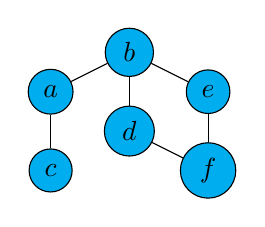
\begin{tikzpicture}
           [dot/.style = {draw,fill=cyan,circle}]
          \node[dot] (b) at (0,0) {$b$};
          \node[dot] (a) at (-1,-0.5) {$a$};
          \node[dot] (c) at (-1,-1.5) {$c$};
          \node[dot] (d) at (0,-1) {$d$};
          \node[dot] (e) at (1,-0.5) {$e$};
          \node[dot] (f) at (1,-1.5) {$f$};
          
          \path[-] (c) edge (a);
          \path[-] (a) edge (b);
          \path[-] (b) edge (e);
          \path[-] (e) edge (f);
          \path[-] (f) edge (d);
          \path[-] (d) edge (b);
        \end{tikzpicture}
    \end{center}
    \newpage
    \item[9.] Draw a graph with:
    \begin{itemize}
        \item[(a)] Four vertices, each with degree 1
        
        \begin{center}
            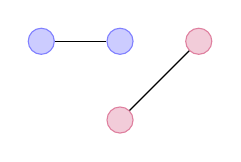
\begin{tikzpicture}[]
               \node (a) at (0,0) [circle, draw=blue!50,fill=blue!20] {};
               \node (b) at (-1,0) [circle, draw=blue!50,fill=blue!20] {};
               \node (c) at (0,-1) [circle, draw=purple!50,fill=purple!20] {};
               \node (d) at (1,0) [circle, draw=purple!50,fill=purple!20] {};
               
               \draw[-] (a) edge (b);
               \draw[-] (c) edge (d);
               
            \end{tikzpicture}
        \end{center}
        
        \item[(b)] Four vertices, each with degree 2
        
        \begin{center}
            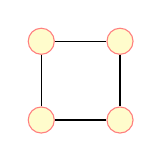
\begin{tikzpicture}[]
               \node (a) at (0,0) [circle, draw=red!50,fill=yellow!20] {};
               \node (b) at (0,-1) [circle, draw=red!50,fill=yellow!20] {};
               \node (c) at (1,0) [circle, draw=red!50,fill=yellow!20] {};
               \node (d) at (1,-1) [circle, draw=red!50,fill=yellow!20] {};
               
               \draw[-] (a) edge (b);
               \draw[-] (c) edge (d);
               \draw[-] (a) edge (c);
               \draw[-] (d) edge (b);
               
            \end{tikzpicture}
        \end{center}
        
        \item[(c)] Four vertices, each with degree 3
        
                \begin{center}
            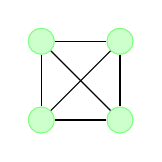
\begin{tikzpicture}[]
               \node (a) at (0,0) [circle, draw=green!50,fill=green!20] {};
               \node (b) at (0,-1) [circle, draw=green!50,fill=green!20] {};
               \node (c) at (1,0) [circle, draw=green!50,fill=green!20] {};
               \node (d) at (1,-1) [circle, draw=green!50,fill=green!20] {};
               
               \draw[-] (a) edge (b);
               \draw[-] (c) edge (d);
               \draw[-] (a) edge (c);
               \draw[-] (d) edge (b);
               \draw[-] (b) edge (c);
               \draw[-] (a) edge (d);
               
            \end{tikzpicture}
        \end{center}
    \end{itemize}
    
    \item[11.] Determine if there is an Euler path/circuit by looking at the degrees of the vertices, if it does find it.
    
    \begin{center}
        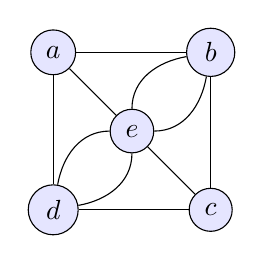
\begin{tikzpicture}
           [dot/.style = {draw,fill=blue!10,circle}]
            \node[dot] (a) at (0, 0) {$a$};
            \node[dot] (b) at (2,0) {$b$};
            \node[dot] (d) at (0,-2) {$d$};
            \node[dot] (c) at (2,-2) {$c$};
            \node[dot] (e) at (1,-1) {$e$};
        
            \path[-] (a) edge (e);
            \path[-] (c) edge (e);
            \path[-] (a) edge (b);
            \path[-] (a) edge (d);
            \path[-] (c) edge (d);
            \path[-] (c) edge (b);
            \path[-] (e) edge[out=180,in=80] (d);
            \path[-] (e) edge[out=270,in=10] (d);
            \path[-] (e) edge[out=90,in=190] (b);
            \path[-] (e) edge[out=0,in=260] (b);
            
            \end{tikzpicture}
    \end{center}
    
    {\color{blue} There is an Euler path, it is: $a,e,b(L),a,d,e(L),d(R),c,b,e(R),c$}
    
    \item[12.] Determine if there is an Euler path/circuit by looking at the degrees of the vertices, if it does find it.
    
    \begin{center}
        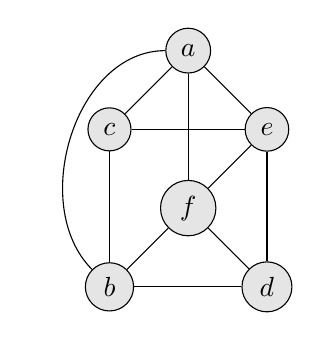
\begin{tikzpicture}
           [dot/.style = {draw,fill=black!10,circle}]
            \node[dot] (a) at (1, 0) {$a$};
            \node[dot] (e) at (2,-1) {$e$};
            \node[dot] (c) at (0,-1) {$c$};
            \node[dot] (b) at (0,-3) {$b$};
            \node[dot] (d) at (2,-3) {$d$};
            \node[dot] (f) at (1,-2) {$f$};
            
            \path[-] (a) edge (c);
            \path[-] (a) edge (e);
            \path[-] (a) edge (f);
            \path[-] (b) edge (c);
            \path[-] (b) edge (f);
            \path[-] (b) edge (d);
            \path[-] (d) edge (f);
            \path[-] (d) edge (e);
            \path[-] (e) edge (f);
            \path[-] (e) edge (c);
            \path[-] (b) edge[out=135,in=180] (a);
            
            \end{tikzpicture}
    \end{center}
    
    {\color{blue} There is an Euler path, it is: $c,a,b,f,d,b,c,e,f,a,e,d$}
    
    \item[15.] Determine if there is a Hamilton path/circuit, explain why not if no path exists.
    
    \begin{center}
        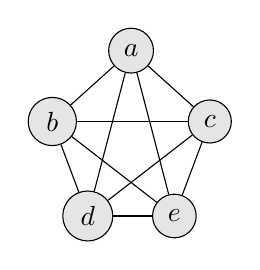
\begin{tikzpicture}
           [dot/.style = {draw,fill=black!10,circle}]
            \node[dot] (a) at (1, 0) {$a$};
            \node[dot] (c) at (2,-0.9) {$c$};
            \node[dot] (b) at (0,-0.9) {$b$};
            \node[dot] (d) at (0.45,-2.1) {$d$};
            \node[dot] (e) at (1.55,-2.1) {$e$};
            
            \path[-] (a) edge (b);
            \path[-] (a) edge (d);
            \path[-] (a) edge (e);
            \path[-] (a) edge (c);
            \path[-] (b) edge (c);
            \path[-] (b) edge (e);
            \path[-] (b) edge (d);
            \path[-] (d) edge (c);
            \path[-] (d) edge (e);
            \path[-] (e) edge (c);
            
            \end{tikzpicture}
    \end{center}
    
    {\color{blue} There is a Hamilton circuit, it is: $a,b,d,e,c,a$}
    
    \newpage
    
    \item[16.] Determine if there is a Hamilton path/circuit, explain why not if no path exists.
    
    \begin{center}
        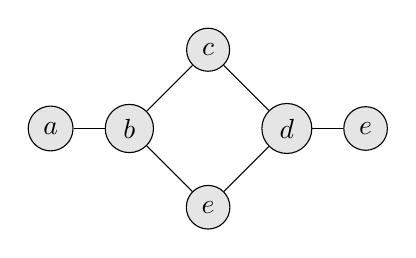
\begin{tikzpicture}
           [dot/.style = {draw,fill=black!10,circle}]
            \node[dot] (a) at (0,0) {$a$};
            \node[dot] (b) at (1,0) {$b$};
            \node[dot] (c) at (2,1) {$c$};
            \node[dot] (e) at (2,-1) {$e$};
            \node[dot] (d) at (3,0) {$d$};
            \node[dot] (f) at (4,0) {$e$};
            
            \path[-] (a) edge (b);
            \path[-] (b) edge (c);
            \path[-] (b) edge (e);
            \path[-] (c) edge (d);
            \path[-] (e) edge (d);
            \path[-] (d) edge (f);
            
            \end{tikzpicture}
    \end{center}
    
    {\color{blue} There is no Hamilton path or circuit because there are diverging paths between $b$ and $d$.}
\end{itemize}

\textbf{Section 4.3}

\begin{itemize}
    \item[1.] Draw graphs that model the situations described in (a) through (c).  After the graphs are drawn, count the number of edges in order to answer the questions posed.
    \begin{itemize}
        \item[(a)] Five executives meet for lunch.  If each executive shakes hands with each other executive, how many handshakes occur?
        
        \begin{center}
        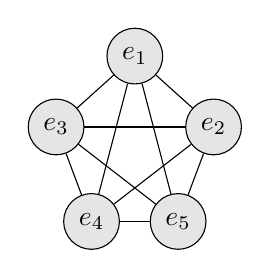
\begin{tikzpicture}
           [dot/.style = {draw,fill=black!10,circle}]
            \node[dot] (a) at (1, 0) {$e_1$};
            \node[dot] (c) at (2,-0.9) {$e_2$};
            \node[dot] (b) at (0,-0.9) {$e_3$};
            \node[dot] (d) at (0.45,-2.1) {$e_4$};
            \node[dot] (e) at (1.55,-2.1) {$e_5$};
            
            \path[-] (a) edge (b);
            \path[-] (a) edge (d);
            \path[-] (a) edge (e);
            \path[-] (a) edge (c);
            \path[-] (b) edge (c);
            \path[-] (b) edge (e);
            \path[-] (b) edge (d);
            \path[-] (d) edge (c);
            \path[-] (d) edge (e);
            \path[-] (e) edge (c);
            
            \end{tikzpicture}
        \end{center}
        
        {\color{blue} There are 10 edges, therefore 10 handshakes occur.}
        
        \item[(b)] Three students rent a single, two seated bicycle.  if each student rides exactly one time with each other student, how many bicycle rides must occur?
        
        \begin{center}
            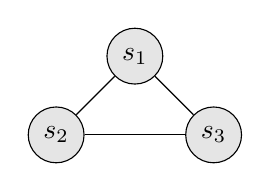
\begin{tikzpicture}
               [dot/.style = {draw,fill=black!10,circle}]
               \node[dot] (s1) at (0,0) {$s_1$};
               \node[dot] (s2) at (-1,-1) {$s_2$};
               \node[dot] (s3) at (1,-1) {$s_3$};
               
               \path[-] (s1) edge (s3);
               \path[-] (s1) edge (s2);
               \path[-] (s2) edge (s3);
            \end{tikzpicture}
        \end{center}
        
        {\color{blue} There are 3 edges, therefore 3 bicycle rides occur.}
        
        \item[(c)] Computers sit on each of four desks, and staff members fro the Information Technology Department design the network so that each pair of computers in connected by a cable.  How many cables must be run to complete the network.
        
        \begin{center}
            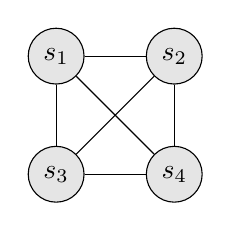
\begin{tikzpicture}
               [dot/.style = {draw,fill=black!10,circle}]
               \node[dot] (c1) at (0,0) {$s_1$};
               \node[dot] (c2) at (1.5,0) {$s_2$};
               \node[dot] (c3) at (0,-1.5) {$s_3$};
               \node[dot] (c4) at (1.5,-1.5) {$s_4$};
               
               \path[-] (c1) edge (c2);
               \path[-] (c1) edge (c3);
               \path[-] (c1) edge (c4);
               \path[-] (c2) edge (c3);
               \path[-] (c2) edge (c4);
               \path[-] (c3) edge (c4);
            \end{tikzpicture}
        \end{center}
        
        {\color{blue} There are 6 edges, therefore 6 cables are needed to complete the network.}
        
        \item[(d)] Each of the graphs drawn in (a) through (c) is an example of what kind of graph?
        
        {\color{blue} These are complete graphs}
    \end{itemize}
    
    \newpage
    
    \item[2.] Draw the complete graphs $K_6$ and $K_7$.
    
    \begin{center}
        $K_6$\\
        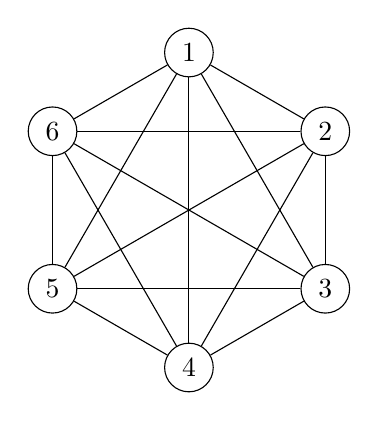
\begin{tikzpicture}[nodes={draw, circle}]
            \graph {subgraph K_n [n=6,clockwise,radius=2cm] };
        \end{tikzpicture}
    \end{center}
    
    \begin{center}
        $K_7$\\
        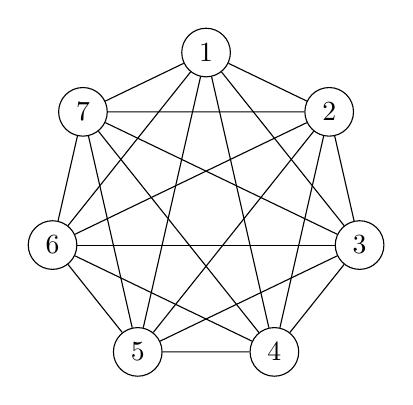
\begin{tikzpicture}[nodes={draw, circle}]
            \graph {subgraph K_n [n=7,clockwise,radius=2cm] };
        \end{tikzpicture}
    \end{center}
    
    \item[3.] Sketch three different subgraphs of graph $G.$ below
    
    \begin{center}
        $G$\\
        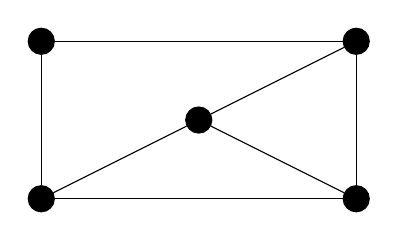
\begin{tikzpicture}
            [dot/.style = {draw,circle,fill=black}]
            \node[dot] (a1) at (0,0) {};
            \node[dot] (a2) at (4,0) {};
            \node[dot] (a3) at (2,-1) {};
            \node[dot] (a4) at (0,-2) {};
            \node[dot] (a5) at (4,-2) {};
            
            \path[-] (a1) edge (a2);
            \path[-] (a1) edge (a4);
            \path[-] (a4) edge (a3);
            \path[-] (a4) edge (a5);
            \path[-] (a3) edge (a2);
            \path[-] (a2) edge (a5);
            \path[-] (a3) edge (a5);
        \end{tikzpicture}
        
        Below are three subgraphs
        
        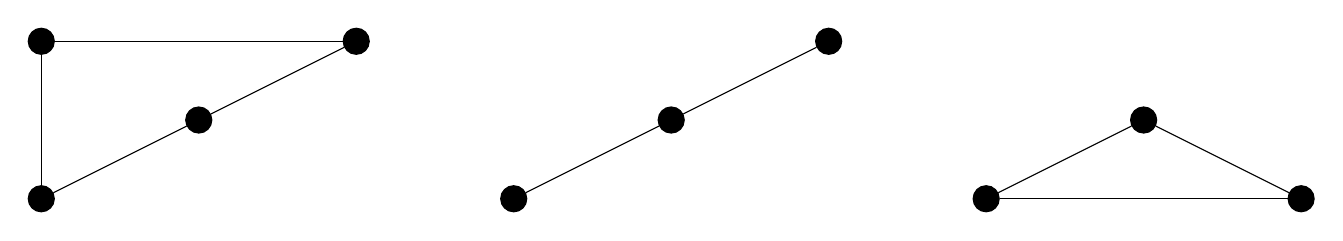
\begin{tikzpicture}
            [dot/.style = {draw,circle,fill=black}]
            \node[dot] (a1) at (0,0) {};
            \node[dot] (a2) at (4,0) {};
            \node[dot] (a3) at (2,-1) {};
            \node[dot] (a4) at (0,-2) {};
            
            \node[dot] (b1) at (6,-2) {};
            \node[dot] (b2) at (8,-1) {};
            \node[dot] (b3) at (10,0) {};
            
            \node[dot] (c1) at (12,-2) {};
            \node[dot] (c2) at (14,-1) {};
            \node[dot] (c3) at (16,-2) {};
            
            \path[-] (a1) edge (a2);
            \path[-] (a2) edge (a3);
            \path[-] (a3) edge (a4);
            \path[-] (a4) edge (a1);
            
            \path[-] (b1) edge (b2);
            \path[-] (b2) edge (b3);
            
            \path[-] (c1) edge (c2);
            \path[-] (c2) edge (c3);
            \path[-] (c3) edge (c1);
        \end{tikzpicture}
    \end{center}
    
    \newpage
    \item[4.] Draw the complete bipartite graphs $K_{3,3}$ and $K_{2,4}$.
    
    \begin{center}
        $K_{3,3}$\\
        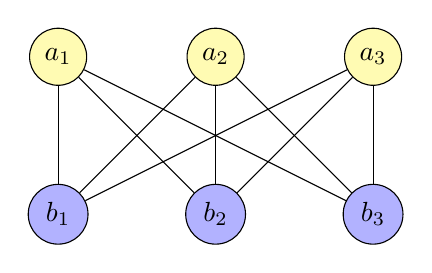
\begin{tikzpicture}
            [dot/.style = {draw,fill=yellow!30,circle},dot2/.style={draw,fill=blue!30,circle}]
            \node[dot] (a1) at (0,0) {$a_1$};
            \node[dot] (a2) at (2,0) {$a_2$};
            \node[dot] (a3) at (4,0) {$a_3$};
            \node[dot2] (b1) at (0,-2) {$b_1$};
            \node[dot2] (b2) at (2,-2) {$b_2$};
            \node[dot2] (b3) at (4,-2) {$b_3$};
            
            \path[-] (a1) edge (b1);
            \path[-] (a1) edge (b2);
            \path[-] (a1) edge (b3);
            \path[-] (a2) edge (b2);
            \path[-] (a2) edge (b3);
            \path[-] (a3) edge (b3);
            \path[-] (a2) edge (b1);
            \path[-] (a3) edge (b1);
            \path[-] (a3) edge (b2);
        \end{tikzpicture}
        
        $K_{2,4}$\\
        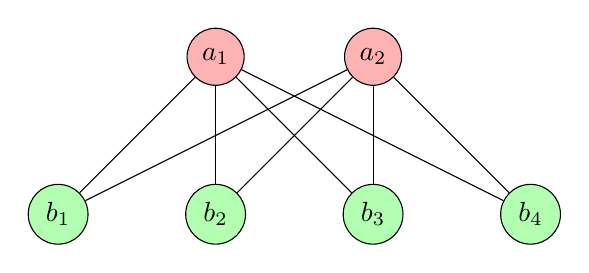
\begin{tikzpicture}
            [dot/.style = {draw,fill=red!30,circle},dot2/.style={draw,fill=green!30,circle}]
            \node[dot] (a1) at (2,0) {$a_1$};
            \node[dot] (a2) at (4,0) {$a_2$};
            \node[dot2] (b1) at (0,-2) {$b_1$};
            \node[dot2] (b2) at (2,-2) {$b_2$};
            \node[dot2] (b3) at (4,-2) {$b_3$};
            \node[dot2] (b4) at (6,-2) {$b_4$};
            
            \path[-] (a1) edge (b1);
            \path[-] (a1) edge (b2);
            \path[-] (a1) edge (b3);
            \path[-] (a1) edge (b4);
            \path[-] (a2) edge (b2);
            \path[-] (a2) edge (b3);
            \path[-] (a2) edge (b1);
            \path[-] (a2) edge (b4);

        \end{tikzpicture}
    \end{center}
    
    For $11-15$ determine  whether the two graphs are isomorphic. If they are, define a one-to-one and onto function between the two vertex sets that preserve the adjacency relationship in both directions.  If the graphs are not isomorphic, describe an invariant property that is not shared by the two graphs.
    
    \item[11.] {\color{blue} These graphs are isomorphic: $a\to z, c\to y, d\to w, b\to w$.}
    
    \item[12.] {\color{blue} These graphs are not isomorphic, vertex $d$ is of degree 3, while no vertices in the other graph have a vertex of degree 3.}
    
    \item[13.] {\color{blue} These graphs are not isomorphic, vertex $e$ is of degree 3, while no vertices in the other graph have a vertex of degree 3. Vertex $a$ is of degree 1, while no other vertices in the other graph have a vertex of degree 1.}
    
    \item[14.] {\color{blue} These graphs are isomorphic: $a\to v, b\to w, c\to x, d\to y, e\to z$.}
    
    \item[15.] {\color{blue} These graphs are not isomorphic, vertices $u$ and $v$ are of degree 2, while there are no vertices in the other graph of degree 2.}
    
    \item[16.] Sketch a complete set of non-isomorphic simple graphs with three vertices.
    
    \begin{center}
        
\begin{tikzpicture}
            [dot/.style = {draw,circle,fill=black}]
            \node[dot] (a1) at (0,0) {};
            \node[dot] (a2) at (0.5,-1) {};
            \node[dot] (a3) at (1,0) {};
            
            \node[dot] (b1) at (2,0) {};
            \node[dot] (b2) at (2.5,-1) {};
            \node[dot] (b3) at (3,0) {};
            
            \node[dot] (c1) at (4,0) {};
            \node[dot] (c2) at (4.5,-1) {};
            \node[dot] (c3) at (5,0) {};
            
            \node[dot] (d1) at (6,0) {};
            \node[dot] (d2) at (6.5,-1) {};
            \node[dot] (d3) at (7,0) {};
            
            \path[-] (b1) edge (b2);
            
            \path[-] (c1) edge (c2);
            \path[-] (c2) edge (c3);
            
            \path[-] (d1) edge (d2);
            \path[-] (d2) edge (d3);
            \path[-] (d3) edge (d1);
        \end{tikzpicture}
    \end{center}
    
    \item[18.] Show that the following graphs are bipartite by finding vertex sets $V_1$ and $V_2$ so that each edge is incident with a vertex in $V_1$ and a vertex in $V_2$.
    \begin{itemize}
        \item[(a)] {\color{blue} $V_1=\{c,d,e\}$ and $V_2=\{a,b\}$}
        
        \item[(b)] {\color{blue} $V_1=\{p,i\}$ and $V_2=\{s,q\}$}
    \end{itemize}
\end{itemize}


\end{document}
